% Search for all the places that say "PUT SOMETHING HERE".

\documentclass[11pt]{article}
\usepackage{amsmath,textcomp,amssymb,geometry,graphicx,enumerate, caption, subcaption, listings}

\def\Name{Aniket Ketkar, Tanay Lathia, Eric Priest, Steve Wang}  % Your name
\def\SID{24795502}  % Your student ID number
\def\Login{aniket.ketkar@berkeley.edu} % Your login (your class account, cs170-xy)
\def\Homework{3} % Number of Homework
\def\Session{Fall 2015}


\title{Statistics 133 - Final Project - ``Team Feelin' the Bern"}
\author{\Name}
\markboth{Stat 133--\Session\  Final Project \Name}{ \Name}
\pagestyle{myheadings}
\date{}

\newenvironment{qparts}{\begin{enumerate}[{(}a{)}]}{\end{enumerate}}
\def\endproofmark{$\Box$}
\newenvironment{proof}{\par{\bf Proof}:}{\endproofmark\smallskip}

\textheight=9in
\textwidth=6.5in
\topmargin=-.75in
\oddsidemargin=0.25in
\evensidemargin=0.25in


\begin{document}
\maketitle
\tableofcontents
\newpage
\section{Abstract}
This project involves the 2016 United States presidential primary races and the role of data in the campaign process.  The goal is to show what ways campaign teams can use election and demographic data to help them properly allocate campaign resources. We predict that through the use of linear regression, we will be able to isolate the main variables that influence voting results and use those variables to create a prediction model for future states. We built a vectorized K Nearest Neighbors (machine learning) model from scratch, running it on the chosen features in the demographic data. We conclude that regression features with KNN produce adequate results for primary voting prediction, with surprising results in homogeneous counties such as Georgia.  


\section{Background}
For the past year, the US Presidential election has consumed the attention of the American people. While many of the publications deal with who said what, the role of data cannot be understated, as we often see polls extrapolated to predict primary results or we see actual election data made into consumer friendly visualizations. With this in mind, our group wanted to look into the different ways data could be used to predict election results and how campaign team behind the scenes could use data. Through Kaggle, we found a data set involving people’s voting patterns in the primaries by county. More specifically, for each county in each state and for each major political party, the data told us the percentage of votes and also the demographic of the people within the county, including features like percentage of each race, average number of households, and percentage of each age range, among many more. The data was sourced from \texttt{https://www.kaggle.com/benhamner/2016-us-election}, compiled by Ben Hamner. See more cleaning details in the Data Analysis Methods section, and \texttt{util.R}. 

\section{Questions for Analysis}
Using this data, we set out to answer these two primary questions:

\begin{enumerate}
	\item[$\cdot$] How can we predict the results for a certain county? 
	\item[$\cdot$] Candidates want to canvass counties that are swing counties, or borderline in terms of votes. Using the data, can we predict which counties would be swing counties based on the features of their demographics?
\end{enumerate}
We chose this idea over others because we wanted to see how we could apply data and the skills we learned in class to modern day relevant issues. Obviously, no one can exactly foresee the outcomes election, but we found the idea of seeing how close we could get to be enticing.
\newpage

\section{Data Analysis Methods}
We obtained the data from Kaggle. The main data files that we used were the “primary\_results.csv” and the “county\_facts.csv” files. The “primary\_results.csv” file gave us data as to how each county voted, for both parties and the “county\_facts.csv” file gave us data as to the demographics of each county. 
The first step we needed to take was to wrangle the data. The data came in the form of three ‘.csv’ files, one that had the election results for each county, one that had the demographic data for each county with the variables in codes, and one that had the key for the variables.  We decided to inner join the county demographic data frame with the election results data frame to create a large data table that had all of the relevant information we wanted to work with. We then created separate data frames for each candidate to get isolated results for each by creating subsets of the large data frame. This separation was helpful later when we ran linear regressions for the candidates.

In order to find the answers to these questions, we needed to slim down which features of the demographics we wanted to analyze. It’d take far too much time to process each of these features so the most efficient method is to find the ones that impacted voting patterns the most. We ran linear regressions between each demographic variable and votes to see which variables correlated the most, and with this analysis we determined that racial variables and the average number of household members were the most influential factors. Once we found the main factors, we were able to make plots that depicted just how much influence those variables had. 

We used K Nearest Neighbors in order to generate predictions based off a feature. KNN is explained more in depth in the next section, but its main purpose is as a classifier. For each state, our training data was every county in the United States minus that state, and we our testing data was every county within the state.

\section{Technical Methods}
\textbf{Technologies used: } 
\begin{enumerate}
\item \texttt{R} scripts
\item \texttt{choroplethr}, \texttt{ggplot2}, \texttt{DataComputing} libraries
\item Github and git, see \texttt{https://github.com/ketkar/election} for commit history
\item \LaTeX for final writeup (see Github for code) 
\item Object oriented programming/abstraction. 
\item Vectorized functions (apply)
\item Caching results using \texttt{.rds} files
\end{enumerate}

\newpage

\section{Exploratory Analysis}
Before we jumped into performing machine learning to predict county results, we created a few visualizations to see any obvious trends in the data. The first is just a very simple pie-chart of how the race was stacking up at the time the data were collected. \\

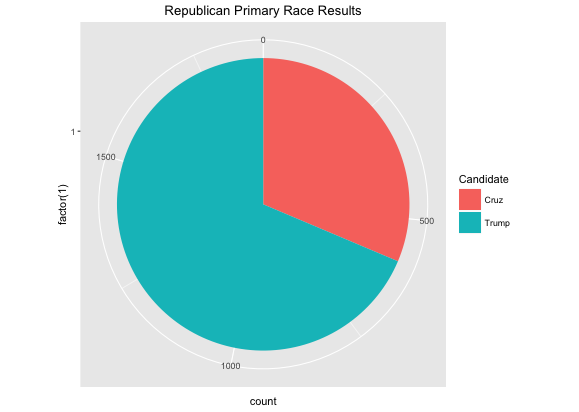
\includegraphics[scale=0.4]{../exploratory_plots/Republican_Primary.png}
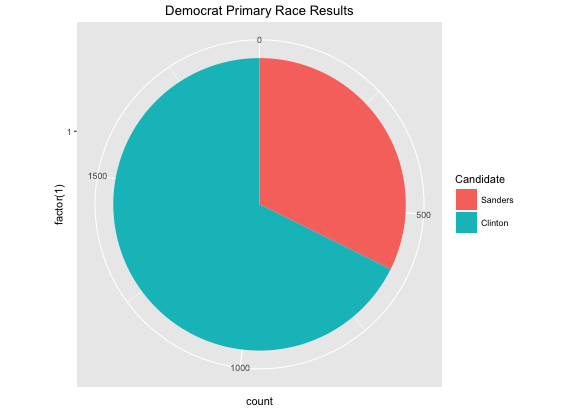
\includegraphics[scale=0.4]{../exploratory_plots/Democrat_Primary.png}

These graphs show the percentage of counties won by each candidate in their respective party. These plots are a great spot to begin our exploratory analysis because firstly they provide a motivation for the analysis: Sanders and Cruz are both on the backfoot in their party races. They need to determine which voter groups they are not hitting and refocus their efforts in order to stand a chance at claiming the nominations. Furthermore, it is important to consider these charts because the skewed nature of the current state of the primaries will bias any results we generate - especially when using K Nearest Neighbors, an unsupervised learning technique. The nature of the this tool, which we will describe in greater detail in the next section, lends itself to following the bias of the data that has already been collected; so, it is important to be fully aware of the biases before extrapolating results for predictions. \\

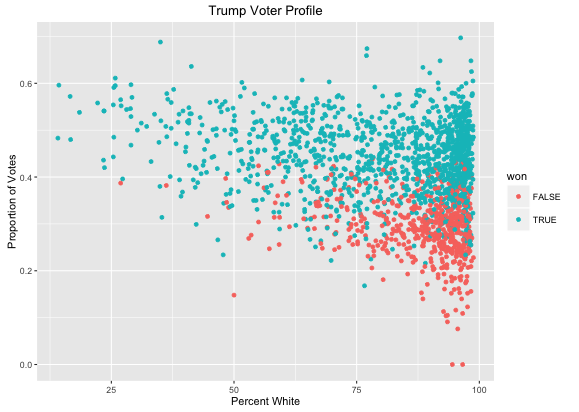
\includegraphics[scale=0.38]{../exploratory_plots/Trump_White.png}
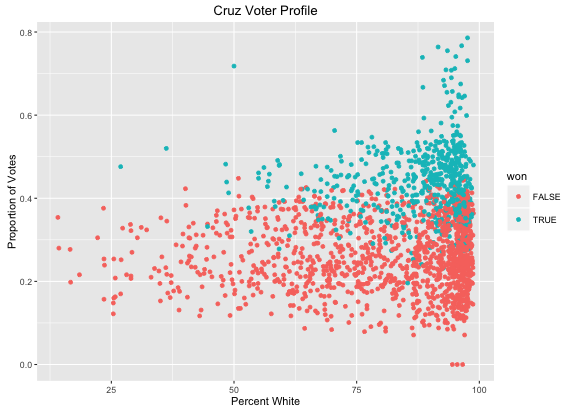
\includegraphics[scale=0.38]{../exploratory_plots/Cruz_White.png}\\
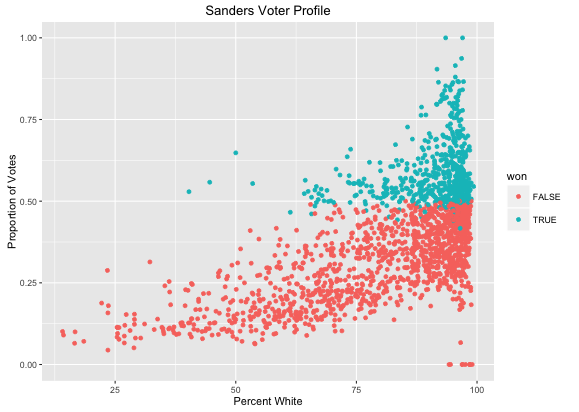
\includegraphics[scale=0.38]{../exploratory_plots/Sanders_White.png}
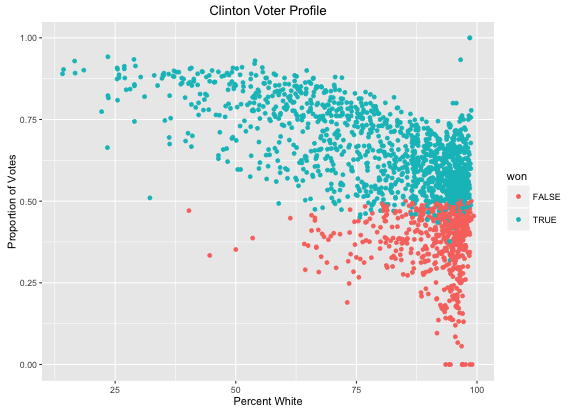
\includegraphics[scale=0.38]{../exploratory_plots/Clinton_White.png}\\

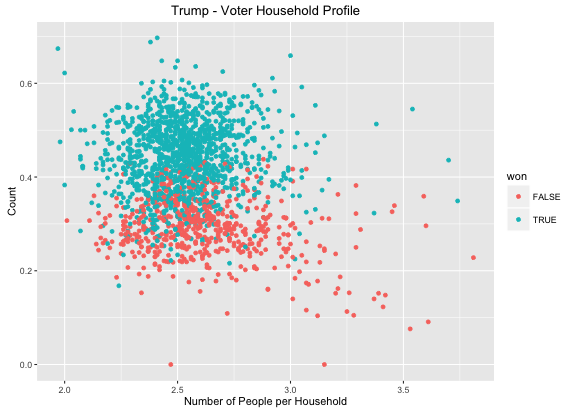
\includegraphics[scale=0.38]{../exploratory_plots/Trump_Num_People.png}
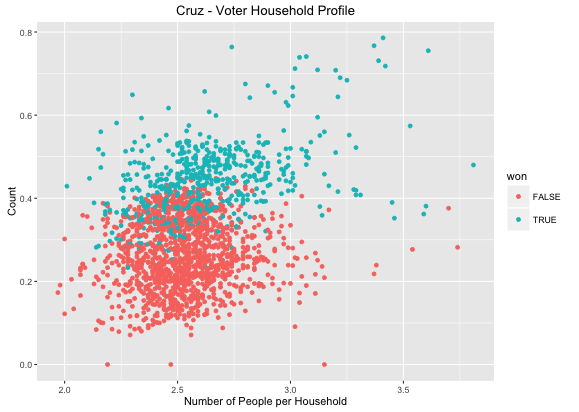
\includegraphics[scale=0.38]{../exploratory_plots/Cruz_Num_People.png}\\
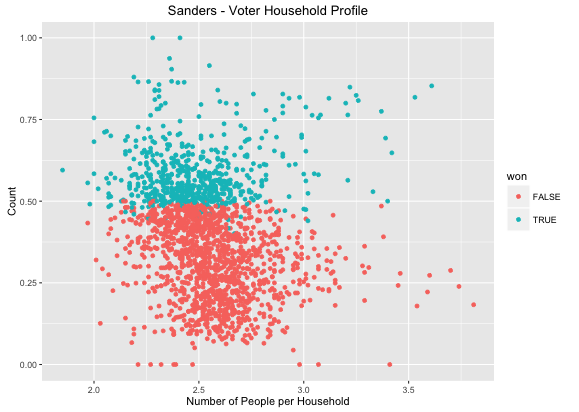
\includegraphics[scale=0.38]{../exploratory_plots/Sanders_Num_People.png}	
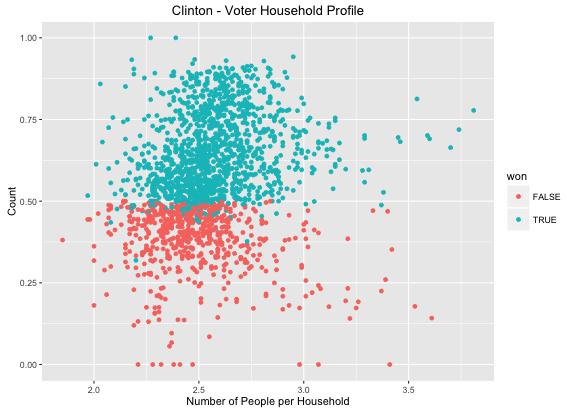
\includegraphics[scale=0.38]{../exploratory_plots/Clinton_Num_People.png}

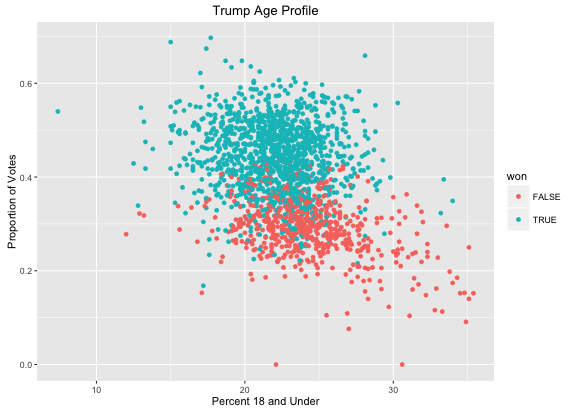
\includegraphics[scale=0.38]{../exploratory_plots/Trump_Age.png}
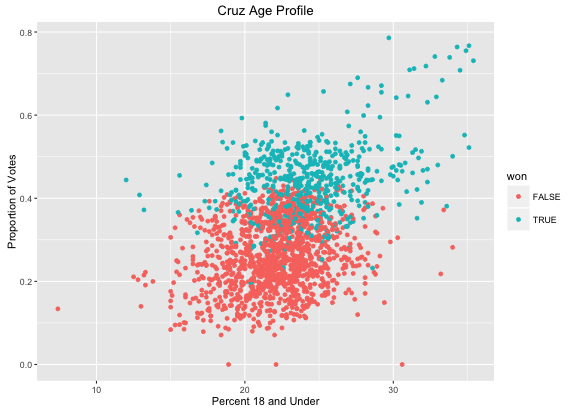
\includegraphics[scale=0.38]{../exploratory_plots/Cruz_Age.png}\\
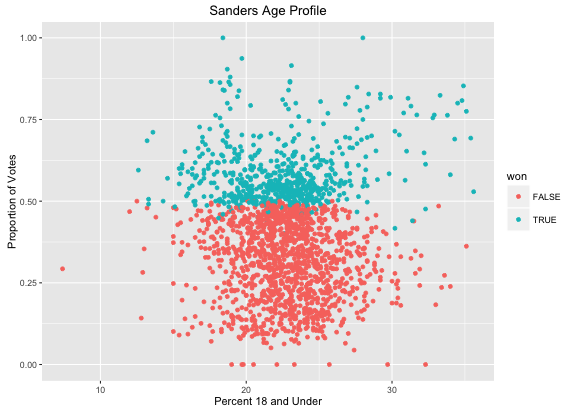
\includegraphics[scale=0.38]{../exploratory_plots/Sanders_Age.png}
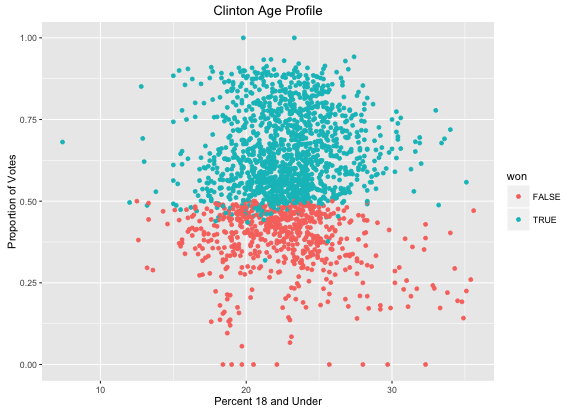
\includegraphics[scale=0.38]{../exploratory_plots/Clinton_Age.png}\\

Despite the shortcomings of KNN, our full exploratory analysis suggested that it made the most sense for us to use in our attempt at classification. Above are a selection of the plots we generated while reviewing the dataset. In every plot, each data point represents a county. The y-axis is always the proportion of votes that the plot's candidate received. The point of interest is always the x-axis which is the feature we were examining. In order from top to bottom, the plots examine how well each candidate does with respect to: proportion of white voters, average number of people per household, and proportion of young voters. Furthermore the plots are organized such that Cruz and Trump are next to each other and Clinton and Sanders are also next to each other in each row. This is so that inter-party comparisons (which are the only valid ones we can make based on this data) are easier. Also, the proportions of voters for Cruz plus Trump add up to 1 (approximately) and the same goes for Sanders and Clinton. This is because only these four candidates got any real traction in the election and this makes our assumption that there are only four candidates in the race.\\

The most compelling plot is the first one - how the proportion of votes received varies with proportion with white voters. We can see that for both Trump and Clinton if there are more than 50\% non-white voters it is very, very likely that they win the county. The county is more of a tossup for counties with more white voters, but seeing this first plot made us hopeful that we could generate a linear classifier. Using just one feature, we can predict very accuracy counties with less than 50\% white voters. However, as we explored more of the features in the data set, we found that no other demographic indicator was nearly as powerful as amount of whites. For example, with number of people per household Cruz seems to have more appeal than Trump for families however this doesn't seem to impact the Democratic race. There is also a similar trend that favors Cruz for younger voters - however it is not nearly as significant as the white voters feature. \\

Because of the limited data separation that we could get from adding more features, we determined that a linear classifier would not do well. The features we had access did not provide enough resolution between certain counties. Because of these limitations, we decided that KNN would be an appropriate model that would be the easiest for us to tune to get accurate results.
\newpage

\section{Machine Learning - K Nearest Neighbors}
\subsection{KNN Equations and Algorithm}
K Nearest neighbors is a nonparametric machine learning technique to find similar points in a dataset. It makes the assumption that similar points will have similar results, so point's label is predicted as the average label of its neighbors. Check out \texttt{knn.R} for the team's implementation of KNN. 
KNN does not make any assumptions about the structure of the dataset, underlying trends, or high level ideas. It just finds the nearest neighbors. For large datasets, like the one in this paper, KNN must run through all of the training points before it can make a prediction. Performance is guaranteed to be linear ($O(nf)$) with the size of the training data $n$ and number of features $f$. The more features, the farther points will be in space due to the curse of dimensionality, so we had to cut down on the featureset to make predictions better. \\ 

Let a single data point be $\mathbf{x_i} = (f_1, f_2, f_3...)$, in entire dataset $\mathbf{X}$. Then for training data point $\mathbf{x_j}$ for $i \neq j$, define the L2 distance metric for a single training example as $t_j = \sqrt{\Sigma(\mathbf{x_i} - \mathbf{x_j})^2}$. The training point $\mathbf{x_j}$ with minimum $t_j$ is the closest example to the desired prediction point. 

The algorithm is: 

\begin{enumerate}
\item For all $j \neq i$, compute $t_j$ 
\item Find $k$ smallest $t_j$ 
\item Return average of these $k$ values. 
\end{enumerate}

As you can see, this involves the entire training set. For state level predictions, we removed the state we are predicting on, leaving approximately 1600 counties to predict on. Each state prediction takes approximately 4 minutes (approximately 20 individual predictions). 

Despite the downsides, KNN performed much better than chance. Assuming two people races, a uniform assumption has expected win rate of 0.5, but every state had at least 70\% success, with some over 90%. 

\subsection{Trump v Cruz Plots}
\textbf{Trump's data worked mostly well with KNN.} Below are some examples of states. The predictions are on the left, the actual results are on the right. Darker blue areas correspond to his predicted wins. See the Analysis section for breakdowns.  \\

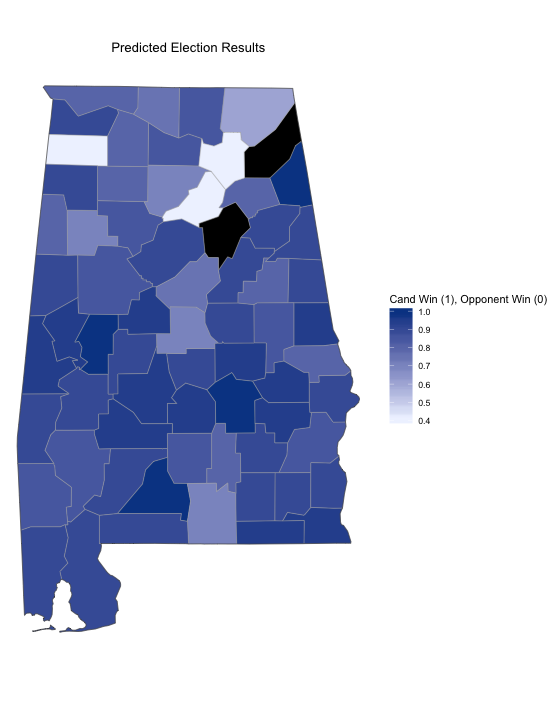
\includegraphics[scale=0.4]{../knn_plots/alabama_predicted.png} 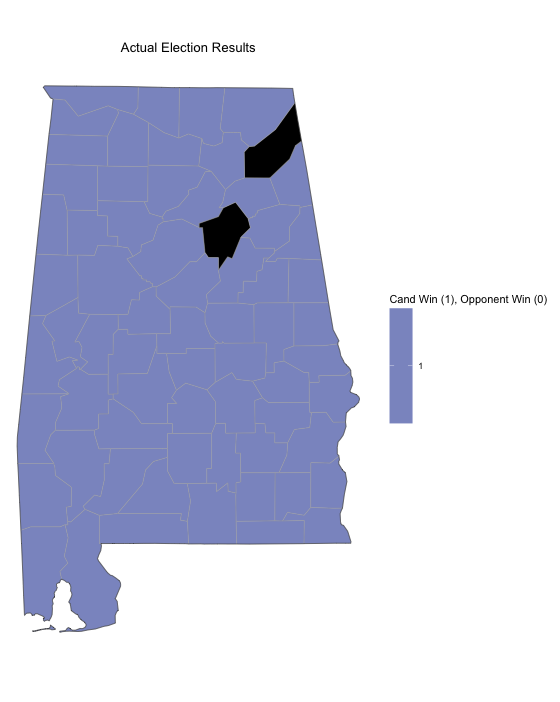
\includegraphics[scale=0.4]{../knn_plots/alabama_actual.png}\\
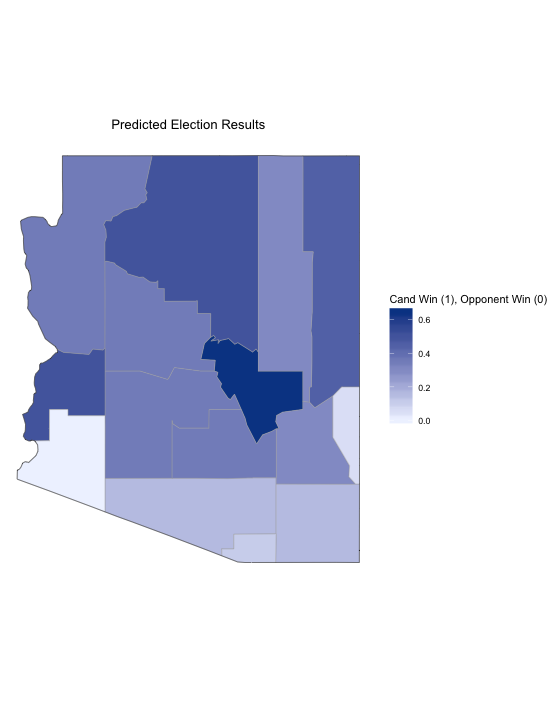
\includegraphics[scale=0.4]{../knn_plots/arizona_predicted.png} 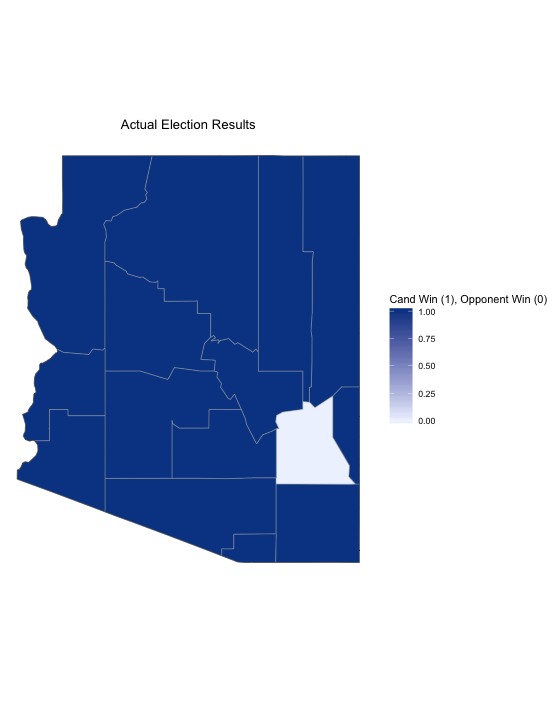
\includegraphics[scale=0.4]{../knn_plots/arizona_actual.png}\\
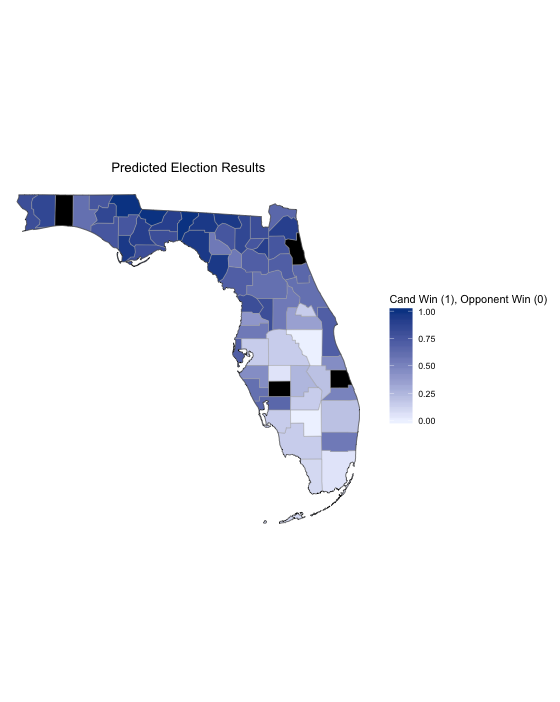
\includegraphics[scale=0.4]{../knn_plots/florida_predicted.png} 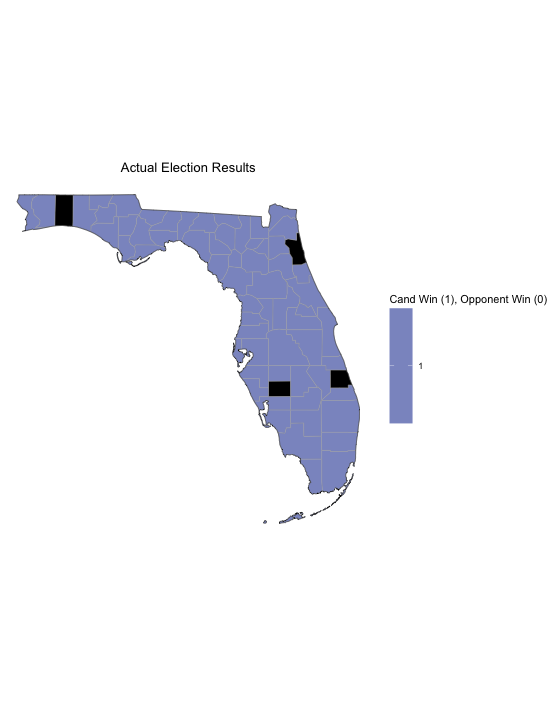
\includegraphics[scale=0.4]{../knn_plots/florida_actual.png}\\
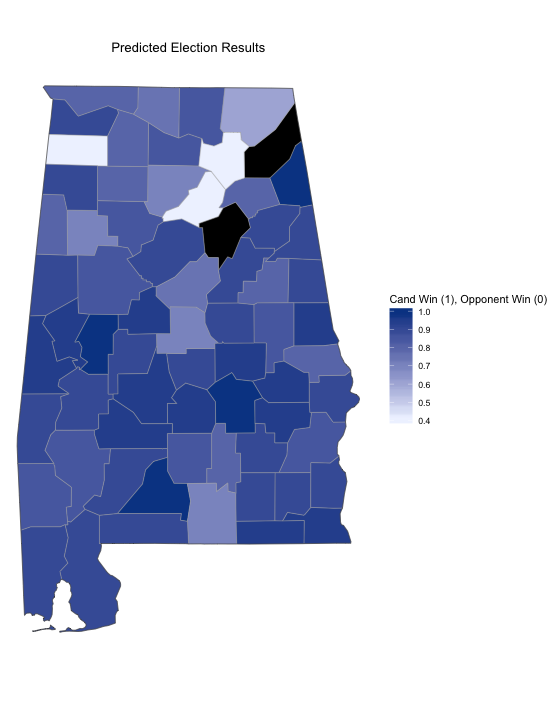
\includegraphics[scale=0.4]{../knn_plots/alabama_predicted.png} 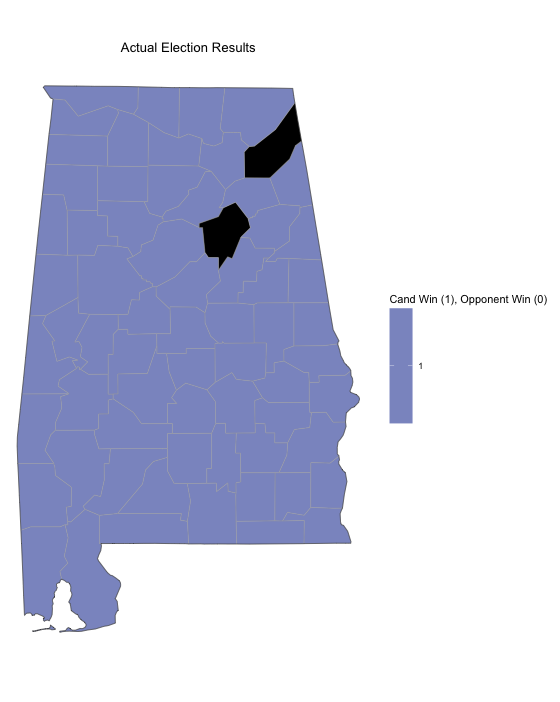
\includegraphics[scale=0.4]{../knn_plots/alabama_actual.png}\\
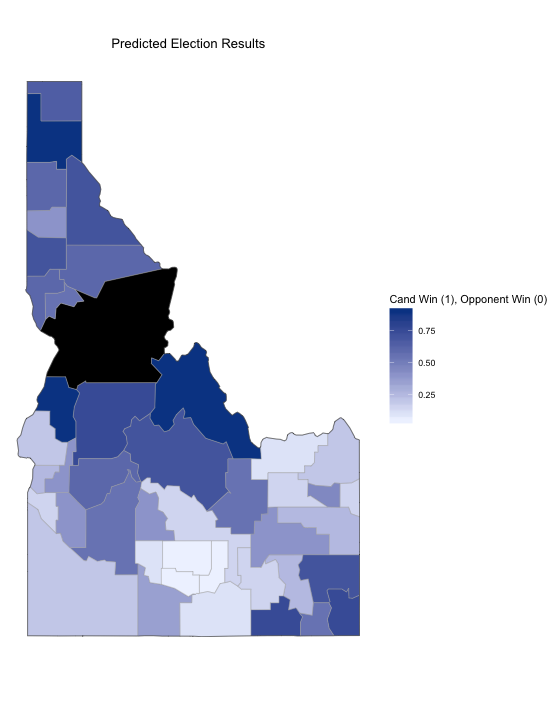
\includegraphics[scale=0.4]{../knn_plots/idaho_predicted.png} 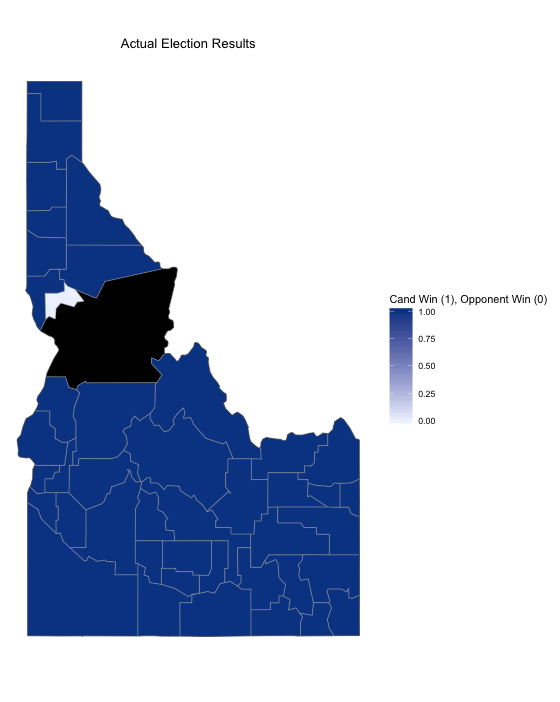
\includegraphics[scale=0.4]{../knn_plots/idaho_actual.png}\\


\subsection{Sanders v Clinton Plots}
\textbf{The model somewhat works for Democratic candidates. } Here are the predictions for Sanders: \\
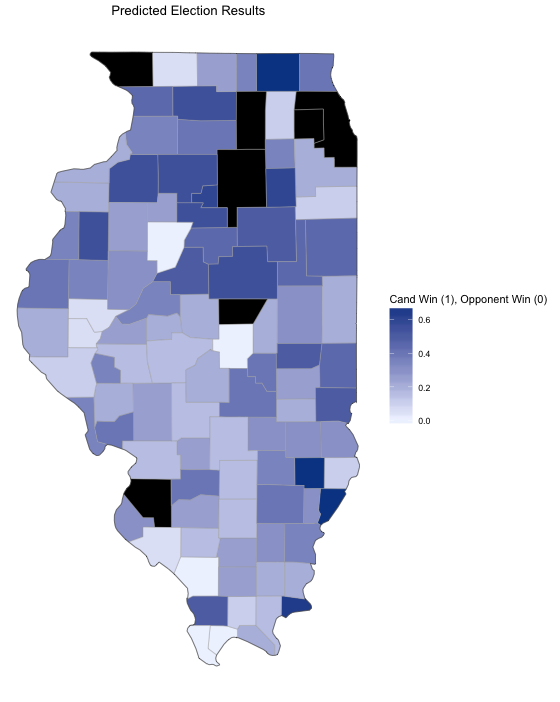
\includegraphics[scale=0.4]{../knn_plots/illinois_predicted.png} 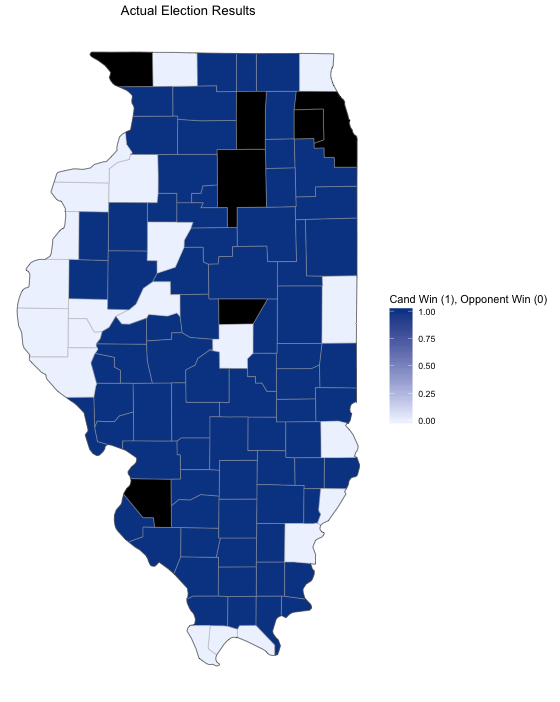
\includegraphics[scale=0.4]{../knn_plots/illinois_actual.png}\\
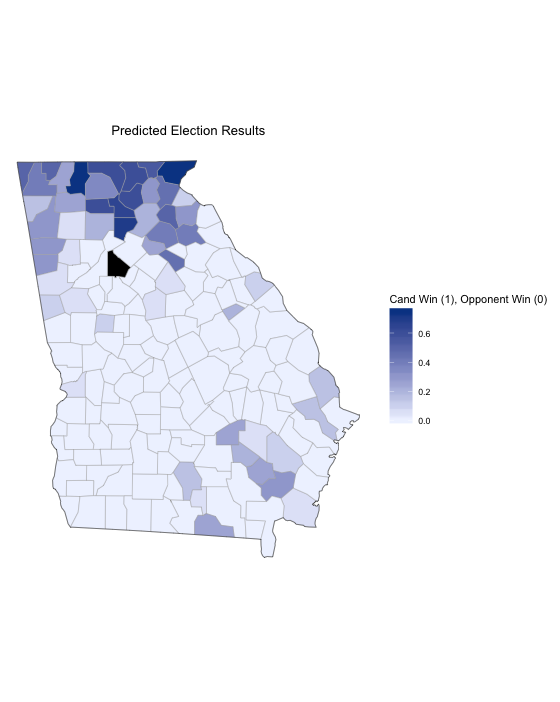
\includegraphics[scale=0.4]{../knn_plots/georgia_sanders_predicted.png} 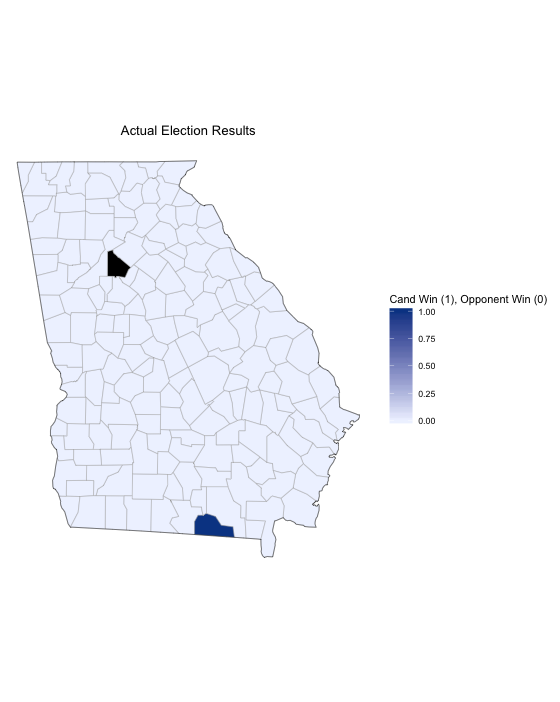
\includegraphics[scale=0.4]{../knn_plots/georgia_sanders_actual.png}\\

\subsection{KNN Analysis}
The model works on a macro scale for each state, correctly predicting the majority of counties. It does well for homogeneous states, or states with clear demographic boundaries. A homogenous example is Sander's overwhelming loss in Georgia, since the counties are small and similar to each other and other Southern Clinton wins. Illinois has high variance between Chicago and other counties, and Northern states split more evenly between Sanders and Clinton, so the neighbors were split as well, leading to poorer performance. 

Some states, like Arizona, Alabama, and Florida, are complete Trump wins. The model does somewhat account for Trump's wins, but it doesn't capture the totality of his wins. The 2016 election is unusual with a rogue candidate, so traditional metrics like demography do not perform as expected in these overwhelming cases. States have many different styles of counties, so it's hard for a model to predict a 100\% Trump win. 

However, KNN performs better in nuanced and battleground states -- in particular in Idaho. Idaho's central regions voted for Trump and the periphery voted for Cruz, and the KNN model accurately captures this pattern. This is a big success for the model -- we predicted the central areas to have Trump tendencies, and they did. The model does a good job because the state had well-known demographic demarcations and was not as affected by Trump hysteria. 

Overall, the model works well when the training data is relatively homogenous. If a candidate has clearly won similar states, the model correctly predicts that they will win future similar states. In addition, if there are clear boundaries within a state, the model will pick up on that fact. However, it does poorly with overwhelming and unusual results, which unfortunately are common in this election. \\

The results confirm that a candidate can expect demographic data to be a good proxy for prediction, but the data do not make perfect predictions. The best performance is for historically strongly voting counties. Novel counties do not perform well with KNN analysis. A candidate should run KNN and canvas in doubtful areas, but not rely completely on the model. We imagine that a candidate will have a good idea of his or her performance, but wants to fine tune their strategy in battleground states like Idaho. The regression-tuned KNN model will be useful in these scenarios. 


\section{Conclusion - Answering the Questions}
We concluded that using even one feature could give us somewhat accurate results. We made predictions solely based on the race and household population demographics of a county. As seen in these side-by-side comparisons of our predicted election results based on a sole feature, we could obtain results that looked fairly close to the actual results. There were some counties that were vastly different, but that is expected in using only a single feature. To answer the question we initially asked, as a whole, \textbf{yes, we can conclude that race and demographic data can be used as a predictor of voting patterns.} In addition, we can use this data to predict which counties are swing counties and if we were a team working to support a specific candidate, we would invest more time and money into these counties to swing things in our favor. Although the model performs poorly with unusual scenarios (Trump), it can be useful in hard fought states. 

This project could be expanded further by using multiple features, and seeing how well we could predict using only five or ten features. Due to limited time and resources, we weren’t able to do it here. Random forests (with decision stumps) is well suited to the data as well, but takes an even longer time to train. Future analysis could include a random forest algorithm running on a more powerful computer. 

\newpage

\section{Code Appendix}
\subsection*{Code Structure}
We went with an abstraction approach, modularizing parts for easy reuse. \texttt{util.R} cleans and organizes the data by joining the county data and candidate data tables, then renaming columns for human-parsable form, and attaching additional labels. This script is imported in every other file, so it was easy to change data formats because of a singular dependency. \texttt{visualizations.R} used \texttt{util.R} to make the exploratory data analysis plots. We implemented from scratch KNN in \texttt{knn.R} and exposed \texttt{knn\_pred()} with multiple arguments for other files to use. Finally, \texttt{map.R} runs the KNN in a mapping function, which can be easily switched to any state in the dataset. The flexibility in the code allows for quick changes to output without major refactoring, so this code is usable to other teams interested in the same topic. RDS files were used to avoid redundant computations. 

\subsection{util.R - Utility Functions and Data Cleaning} 
\lstinputlisting[language=R, breaklines=true, numbers=left]{../util.R}
\newpage
\subsection{visualizations.R - Exploratory Data Analysis} 
\lstinputlisting[language=R, breaklines=true, numbers=left]{../visualizations.R}
\newpage
\subsection{knn.R - From scratch KNN Implementation (using apply!)} 
\lstinputlisting[language=R, breaklines=true, numbers=left]{../knn.R}
\newpage
\subsection{map.R - Running KNN and Mapping Results} 
\lstinputlisting[language=R, breaklines=true, numbers=left]{../map.R}
\end{document}
